\section{Example: Traffic Sign Recognition}

\begin{frame}
	\frametitle{Trafficsign-Recognition}
	\framesubtitle{Explaining a neural network}
	\begin{Large}
		given neural network :
		\begin{itemize}
				\item 6 layers, first 3 convolutional (complex structure)
				\item 43 Classes (complex output)
				\item 64x64 Images (complex input) 
				\item trained with 8k images (rich data-input)
				\item tested with 2k images reaching 95\% accuracy (good?)
		\end{itemize}
	\end{Large}
	The NN was trained with Tensorflow and is shipped with your notebook. 
\end{frame}

\begin{frame}
	\frametitle{Trafficsign-Recognition}
	\framesubtitle{How to}
	\lstinputlisting{TexFiles/LimeSnippet.py}
\end{frame}

\begin{frame}
	\frametitle{Trafficsign-Recognition}
	\framesubtitle{Simple Classification}
	
	\begin{columns}
		\begin{column}{0.33\textwidth}
			\begin{center}
				\begin{figure}[H]
					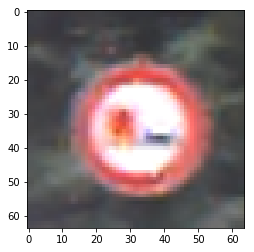
\includegraphics[width=0.9\linewidth]{Images/NoOvertaking}
					\caption[No Overtaking]{No Overtaking - Sample Image from Test-data}
					\label{fig:noovertaking}
				\end{figure}
			\end{center}		
		\end{column}
		\begin{column}{0.33\textwidth}
			\begin{center}
				\begin{figure}[H]
					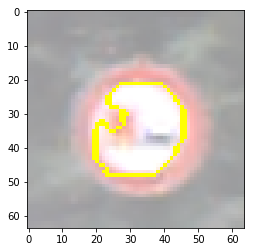
\includegraphics[width=0.9\linewidth]{Images/NoOvertakingCorrectClass}
					\caption[Prediction:  No Overtaking]{ Prediction - showing the 5 Superpixels for \textit{no overtaking}}
					\label{fig:noovertakingCorrect}
				\end{figure}
			\end{center}
		\end{column}
		\begin{column}{0.33\textwidth}
		\begin{center}
			\begin{figure}[H]
				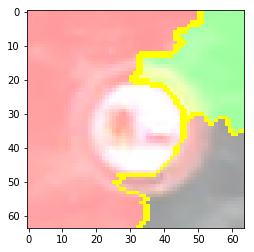
\includegraphics[width=0.9\linewidth]{Images/NoOvertakingFalseClass}
				\caption[Prediction:  right of way crossing]{ Prediction - showing the 4 most important Superpixels for \textit{right of way crossing}}
				\label{fig:noovertakingFalse}
			\end{figure}
		\end{center}
		\end{column}
	\end{columns}
\end{frame}

\begin{frame}
	\frametitle{Trafficsign-Recognition}
	\framesubtitle{Overfitting}
	\begin{columns}
		\begin{column}{0.33\textwidth}
			\begin{center}
				\begin{figure}
					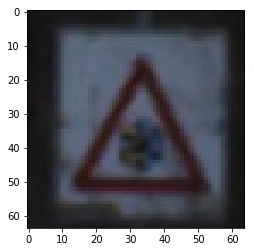
\includegraphics[width=0.9\linewidth]{Images/Frost}
					\caption[Frost]{Frost - Sample Image from \textit{Training}-data}
					\label{fig:frost}
				\end{figure}
			\end{center}		
		\end{column}
		\begin{column}{0.33\textwidth}
			\begin{center}
				\begin{figure}
					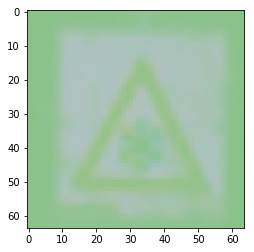
\includegraphics[width=0.9\linewidth]{Images/FrostOverfitting}
					\caption[Prediction:  Frost]{ Prediction for \textit{Frost}, a sign for overfitting}
					\label{fig:frostOverfit}
				\end{figure}
			\end{center}
		\end{column}
	\end{columns}
\end{frame}

\begin{frame}
	\frametitle{Trafficsign-Recognition}
	\framesubtitle{Similiar Classes I}
	\begin{columns}
		\begin{column}{0.33\textwidth}
			\begin{center}
				\begin{figure}
					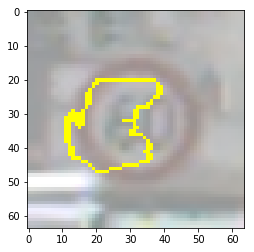
\includegraphics[width=0.9\linewidth]{Images/60Prediction}
					\caption[60]{Prediction: 60 - only 6 is circled}
					\label{fig:60Pred}
				\end{figure}
			\end{center}		
		\end{column}
		\begin{column}{0.33\textwidth}
			\begin{center}
				\begin{figure}
					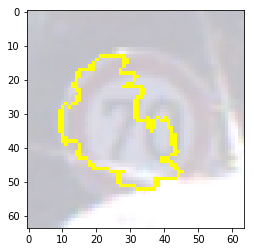
\includegraphics[width=0.9\linewidth]{Images/70Prediction}
					\caption[70]{Prediction: 70 - only 7 is circled}
					\label{fig:70Pred}
				\end{figure}
			\end{center}
		\end{column}
	\end{columns}
	\begin{center}	
		\textbf{The model seems to recognize numbers!}
	\end{center}
\end{frame}

\begin{frame}
\frametitle{Trafficsign-Recognition}
\framesubtitle{Similiar Classes II}
\begin{center}	
	Let's have some fun!
\end{center}
\begin{columns}
	\begin{column}{0.33\textwidth}
		\begin{center}
			\begin{figure}
				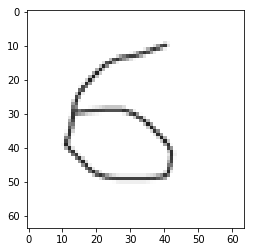
\includegraphics[width=0.9\linewidth]{Images/6Image}
				\caption[6]{Only number 6, no Street Sign}
				\label{fig:6}
			\end{figure}
		\end{center}		
	\end{column}
	\begin{column}{0.33\textwidth}
		\begin{center}
			\begin{figure}
				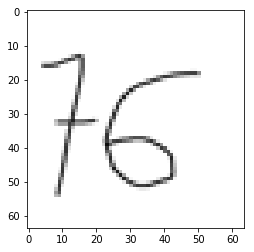
\includegraphics[width=0.9\linewidth]{Images/76Image}
				\caption[76]{Number 76 - what will be predicted?}
				\label{fig:76}
			\end{figure}
		\end{center}
	\end{column}
\end{columns}
\end{frame}

\begin{frame}
\frametitle{Trafficsign-Recognition}
\framesubtitle{Similiar Classes III}
\begin{center}	
	Let's have some fun!
\end{center}
\begin{columns}
	\begin{column}{0.33\textwidth}
		\begin{center}
			\begin{figure}
				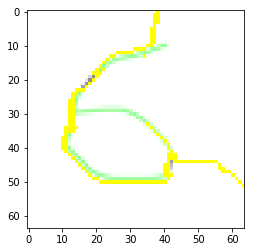
\includegraphics[width=0.9\linewidth]{Images/6Prediction}
				\caption[6]{Number  6  - ~~~ 78\% \textit{Speed Limit 60}}
				\label{fig:6Pred}
			\end{figure}
		\end{center}		
	\end{column}
	\begin{column}{0.33\textwidth}
		\begin{center}
			\begin{figure}
				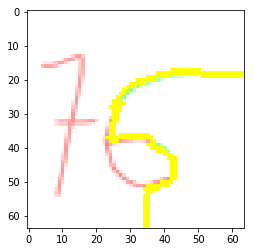
\includegraphics[width=0.9\linewidth]{Images/76Prediction}
				\caption[76]{Number 76 - 99.9\% \textit{No Overtaking}}
				\label{fig:76Pred}
			\end{figure}
		\end{center}
	\end{column}
\end{columns}
\end{frame}

\begin{frame}
	\frametitle{Trafficsign-Recognition}
	\framesubtitle{Conclusion}
	\begin{LARGE}
		\begin{itemize}
			\item Accuracy $\neq$ Quality
			\item most of the predictions \textit{look good}
			\item trainings-data is heavily overfitted
			\item everything that is not a streetsign causes trouble
			\item there can (still) be much more \textit{hidden} problems
		\end{itemize}
	\end{LARGE}
\end{frame}